Modela proste kamere(pinhole) je idealiziran matematični opis razmerja med tridimenzionalnim prostorom in dvodimenzionalno projekcijo slike. Pinhole kamera je sestavljena iz majhne odprtine (pinhole) in slikovne ravnine. Ker se odprtina nahaja med slikovno ravnino in 3D svetom, mora vsak žarek, ki izvira iz 3D prostora, preiti skozi odprtino, preden doseže slikovno ravnino. V tem primeru je projicirana slika obrnjena (\ref{fig:obscura}a). Ta naravni pojav se imenuje kamera obskura in je bil uporabljen skozi zgodovino, opisal pa ga je Ibn al-Haytham v 10. stoletju. Če pa pred odprtino postavimo ravnino, projicirana slika ne bo obrnjena (\ref{fig:obscura}b). 

\begin{figure}[h]
    \centering
    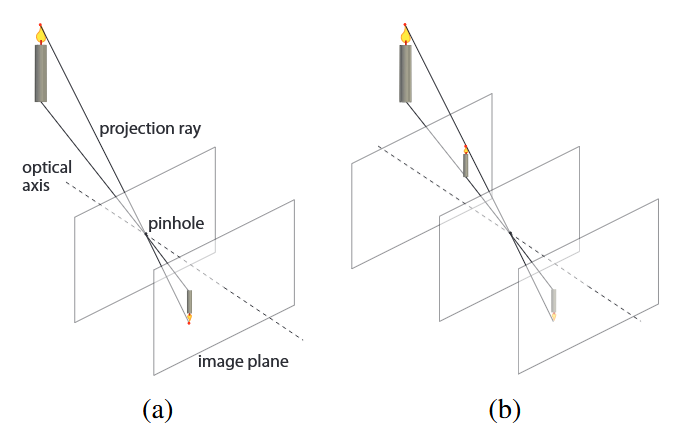
\includegraphics[width=0.5\linewidth]{imgs/obscura.png}
    \caption{Pinhole kamera\cite{Tomasi_2025a}}
    \label{fig:obscura}
\end{figure}

Za matematično razumevanje tega modela moramo najprej definirati 2 pomembna koordinatna sistema\cite{Cyganek_Siebert_2010}. To so:
\begin{itemize}
    \item Zunanji koordinatni sistem('W' za 'world') z izhodišče $\pmb{O_W}$ in osmi $[X_W, Y_W, Z_W]$
    \item Kamera koordinatni sistem('C' za 'camera') z izhodišče $\pmb{O_C}$ in osmi $[X_C, Y_C, Z_C]$
\end{itemize}



\begin{figure}[h]
    \centering
    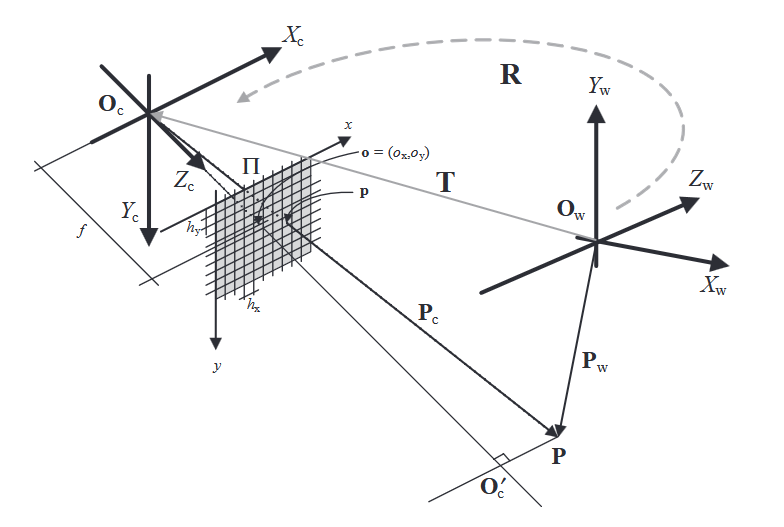
\includegraphics[width=0.8\linewidth]{imgs/pinholemodel.png}
    \caption{Koordinatni sistemi in točke v pinhole kamera\cite{Cyganek_Siebert_2010}}
    \label{fig:pinhole}
\end{figure}

Ta dva koordinatna sistema sta povezana z translacijo $\pmb{t}$ in rotacijo $\pmb{R}$. \\
Naslednje točke lahko vidite na sliki \ref{fig:pinhole}. \\
Slikovna ravnina $\pmb{\Pi}$ je razrezana v pravokotnike, imenovane piksli. Piksli v kameri tvorijo diskretna mesta za zaznavanje fotografije, ki vzorčijo katero koli sliko, projicirano na ravnino. Vsak piksel je indeksiran s parom koordinat, izraženih z naravnimi številkami. $h_x$ in $h_y$ določata fizične dimenzije ene piksle. \\
Točka $\pmb{O_C}$, se imenuje goriščna točka. Njena projekcija na $\pmb{\Pi}$ v smeri $Z_C$ določa glavno točko $o$ na slikovni ravnini. Razdalja od goriščne točke $\pmb{O_C}$ do glavne točke $o$ se imenuje goriščna razdalja $f$. $Z_C$ se imenuje tudi glavna os. Na njej ležijo $\pmb{O_C}$, $o$ in $\pmb{O_C'}$.\\
V realnem svetu lahko določimo neko točko $\pmb{P}$, njen položaj pa je podan z izbranim koordinatnim sistemom, $\pmb{P_C}$ za koordinatni sistem kamere ali $\pmb{P_W}$ za zunanji koordinatni sistem. \\
Točka $\pmb{p}$ je slika točke $\pmb{P}$ na slikovno ravnino s središčem $\pmb{O_C}$. Njihove koordinate lahko definiramo kot:
\[
    \pmb{P} = [X, Y, Z]^T  \qquad \pmb{p} = [x, y, z]^T
\]
Ker imamo podobna trikotnika $\triangle\pmb{O_C p o}$ in $\triangle\pmb{O_C P O_C'}$ dobimo:
\[
    x=f\frac{X}{Z} \qquad y=f\frac{Y}{Z} \qquad z =f
\]
Model pinhole kamere lahko definiramo z dvema skupinama parametrov:
\begin{itemize}
    \item Zunanji parametri(extrinsic)
    \item Notranji parametri(intrinsic)
\end{itemize}